\documentclass{article}

\usepackage{graphicx}
\usepackage{tikz}
\usepackage{tikzsymbols}
\usetikzlibrary{calc,patterns,shapes.geometric}
\pagestyle{empty}
\usepackage[margin=0pt]{geometry}
\geometry{papersize={14in,12in}}

\def\centerarc[#1](#2)(#3:#4:#5){\draw[#1] ($(#2)+({#5*cos(#3)},{#5*sin(#3)})$) arc (#3:#4:#5);}

\begin{document}
	\begin{figure}
		\centering
		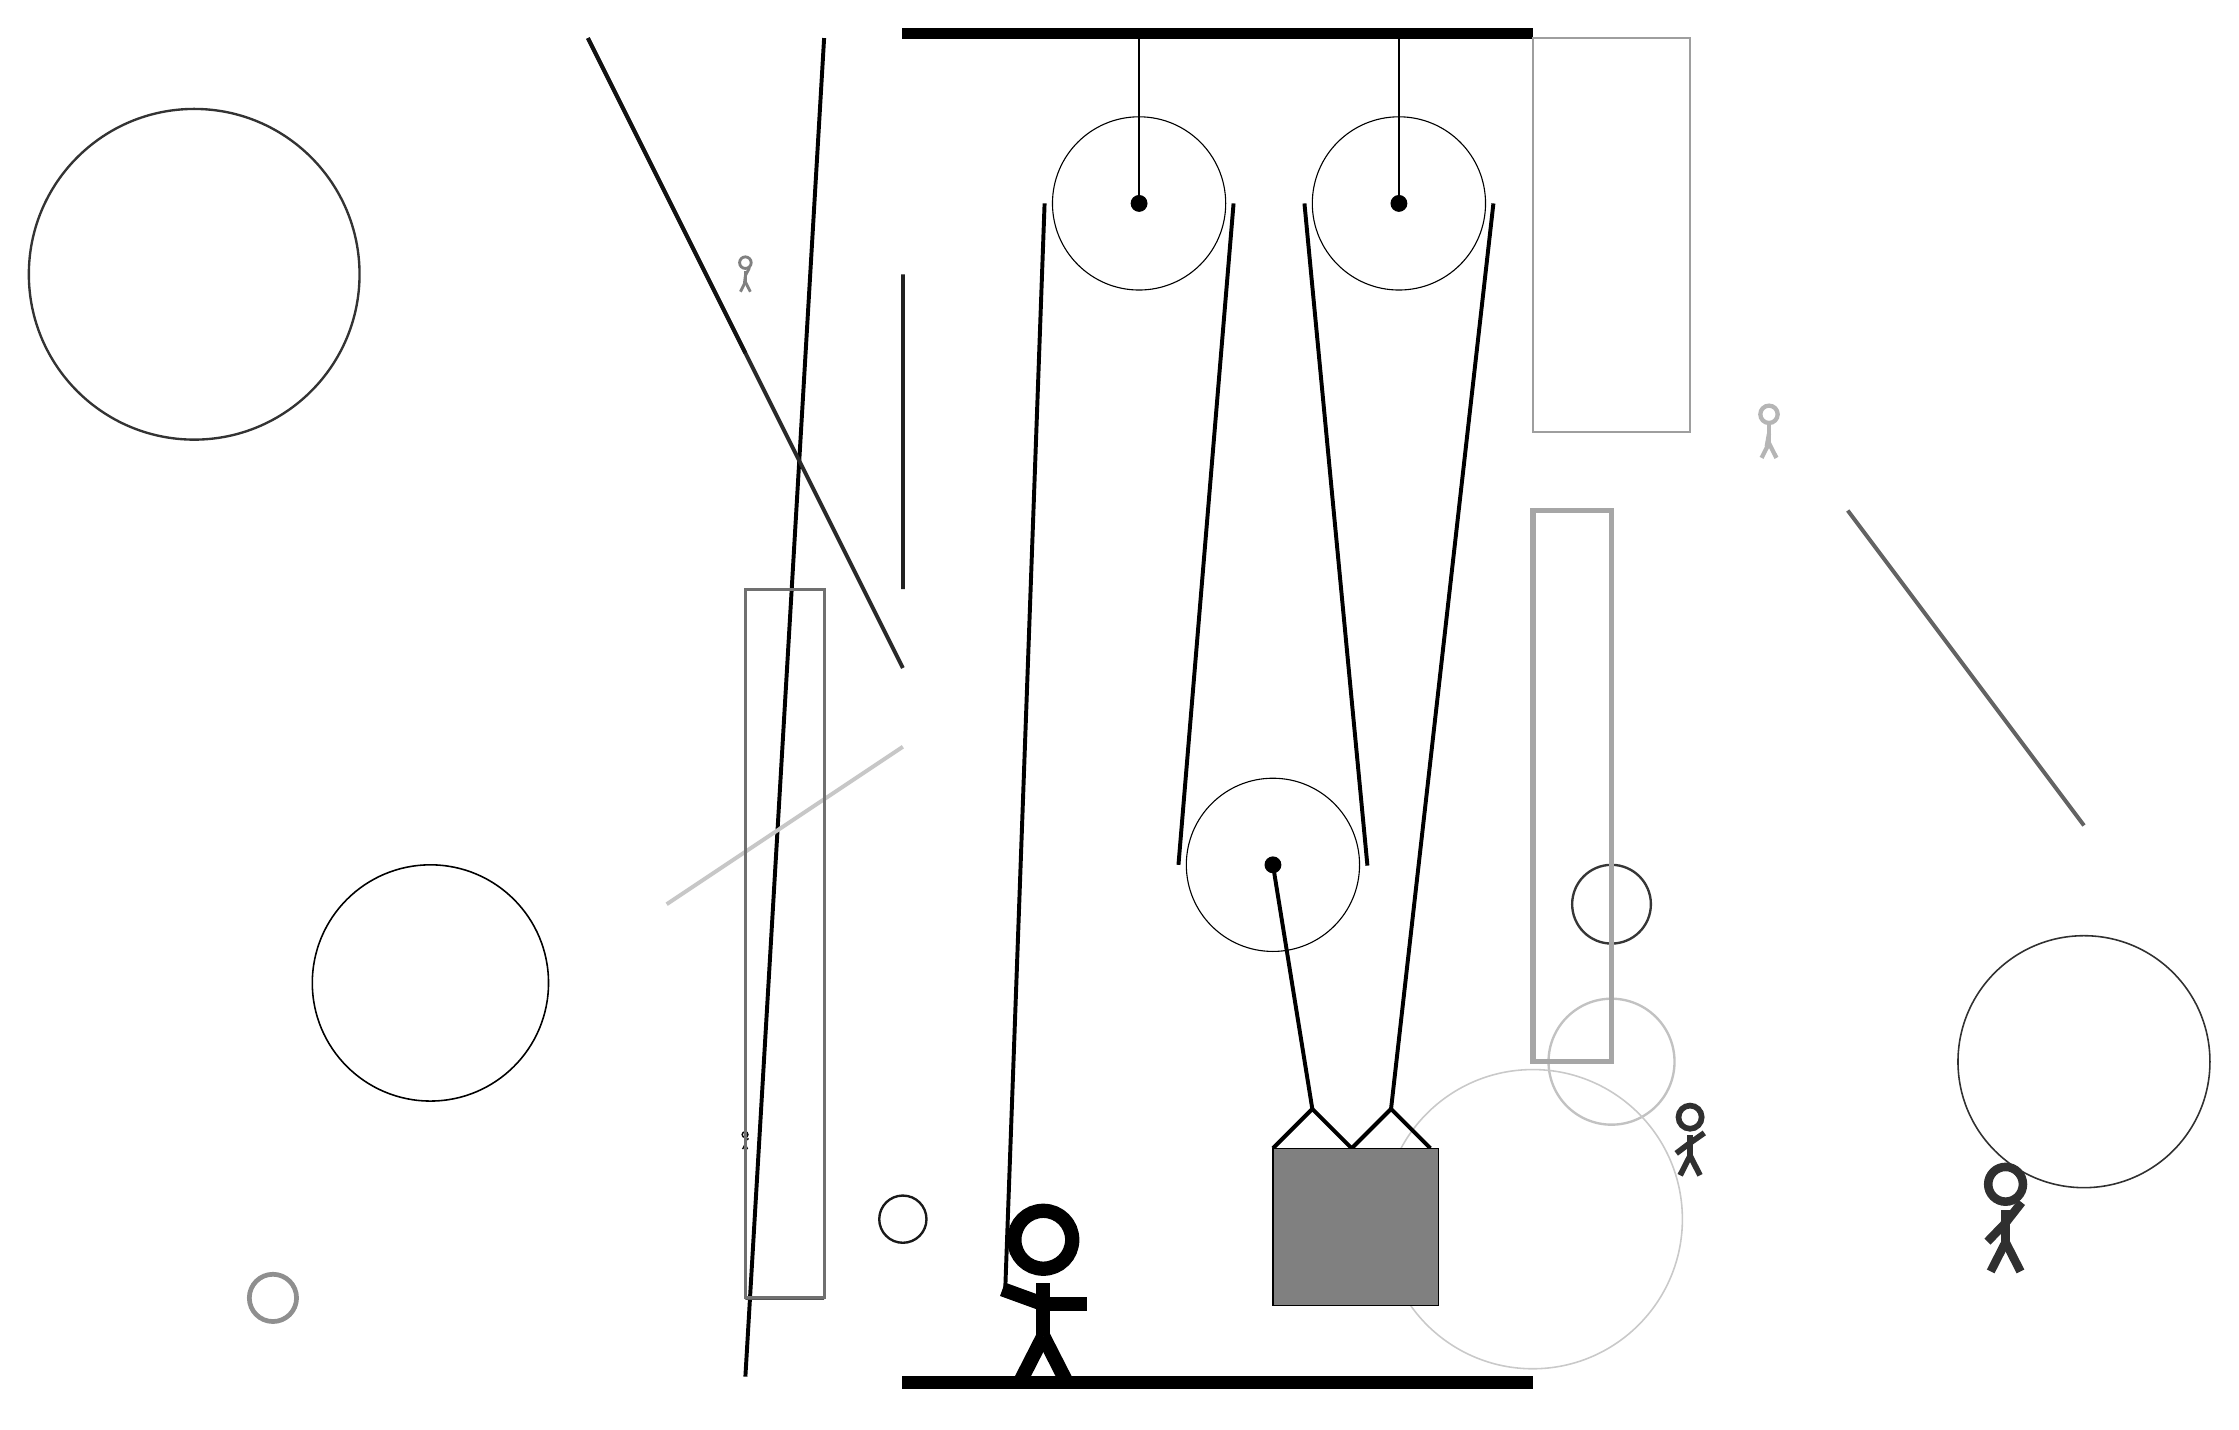
\begin{tikzpicture}
			%%%%% START %%%%%
			
			\draw[fill=black] (-2, 14) rectangle (6, 14.125);
			
			\draw (1, 11.9) circle (1.1);
			\draw[fill=black] (1, 11.9) circle (0.1);
			\draw[thick] (1, 11.9) -- (1, 14);
			
			\draw (4.3, 11.9) circle (1.1);
			\draw[fill=black] (4.3, 11.9) circle (0.1);
			\draw[thick] (4.3, 11.9) -- (4.3, 14);
			
			\draw[line width=0.5mm, color=black!100](-4, -3) -- (-3, 14);
			
			\draw [line width=0.3mm, color=black!79](7, 3) circle (0.5);
			\draw [line width=0.3mm, color=black!24](7, 1) circle (0.8);
			\draw [line width=0.6mm, color=black!44](-10, -2) circle (0.3);
			\draw [line width=0.5mm, color=black!23](-3, -1) circle (0.0);
			\draw[line width=0.5mm, color=black!61](10, 8) -- (13, 4);
			\draw[line width=0.6mm, color=black!87] (-2, 7) rectangle (-2, 11);
			\draw [line width=0.3mm, color=black!90](-2, -1) circle (0.3);
			\draw [line width=0.2mm, color=black!100](-8, 2) circle (1.5);
			\draw[line width=0.5mm, color=black!84](-2, 6) -- (-6, 14);
			\node[line width=0.3mm, color=black!50] at (-4, 11) {\Strichmaxerl[2][83][62]};
			\draw[line width=0.3mm, color=black!38] (6, 14) rectangle (8, 9);
			\node[line width=0.3mm, color=black!97] at (-4, 0) {\Strichmaxerl[1][85][36]};
			
			\node[line width=0.7mm, color=black!81] at (8, 0) {\Strichmaxerl[4][37][35]};
			\draw [line width=0.3mm, color=black!80](-11, 11) circle (2.1);
			\draw [line width=0.2mm, color=black!21](6, -1) circle (1.9);
			\draw[line width=0.6mm, color=black!67] (-4, -2) rectangle (-3, -2);
			\draw[line width=0.5mm, color=black!22](-2, 5) -- (-5, 3);
			\draw [line width=0.2mm, color=black!81](13, 1) circle (1.6);
			\node[line width=0.7mm, color=black!81] at (12, -1) {\Strichmaxerl[6][46][52]};
			\node[line width=0.4mm, color=black!29] at (9, 9) {\Strichmaxerl[3][80][90]};
			
			\draw[line width=0.5mm, color=black!93](-4, 10) -- (-6, 14);
			\draw[line width=0.4mm, color=black!56] (-4, -2) rectangle (-3, 7);
			\draw[line width=0.7mm, color=black!35] (7, 1) rectangle (6, 8);
			
			\draw (2.7, 3.5) circle (1.1);
			\draw[fill=black] (2.7, 3.5) circle (0.1);
			
			\draw[line width=0.5mm]  (2.7, -0.1) -- (3.2, 0.4) -- (3.7, -0.1) -- (4.2, 0.4) -- (4.7, -0.1);
			\draw[fill=black!50] (2.7, -0.1) rectangle (4.8, -2.1);
			
			\draw[line width=0.5mm](-0.7, -1.9) -- (-0.2, 11.9);
			\centerarc[line width=0.5mm](1, 11.9)(0:180:1.2000000000000002);
			\draw[line width=0.5mm](2.2, 11.9) -- (1.5, 3.5);
			\centerarc[line width=0.5mm](2.7, 3.5)(180:370:1.2000000000000002);
			\draw[line width=0.5mm] (3.9, 3.49) -- (3.1, 11.9);
			\centerarc[line width=0.5mm](4.3, 11.9)(0:180:1.2000000000000002);
			\draw[line width=0.5mm](4.2, 0.4) -- (5.5, 11.9);
			\draw[line width=0.5mm] (3.2, 0.4) -- (2.7, 3.5);
			
			\node at (-0.2, -2) {\Strichmaxerl[10][-20][0]};
			
			\draw[fill=black] (-2, -3) rectangle (6, -3.15);
			
			%%%%% END %%%%%
		\end{tikzpicture}
	\end{figure}	
\end{document}